-\section{Experiment}

We conduct experiments under two distinct training paradigms, ``AR to Diffusion'' and ``Training Diffusion from Scratch'', to comprehensively evaluate our proposed method.

\subsection{AR to Diffusion}

For \textbf{AR to Diffusion} experiments, we adopt the experimental settings and framework from Fast-dLLM v2~\citep{fastdllmv2} and use it as our baseline to evaluate the performance gains achieved by our proposed improvements.

\paragraph{Models}

We initialize our model from Qwen2.5-1.5B-Instruct~\citep{qwen2.5} and fine-tune it into a block diffusion language model following the training recipe of Fast-dLLM v2~\citep{fastdllmv2}.
The fine-tuning is performed on approximately 3B tokens sampled from the LLaMA-Nemotron post-training dataset~\citep{nemotronpost}.
The block size $B$ is set to 32, the batch size is set to $256$ and the context length is set to $2048$.
The learning rate is set to $2e-5$.

\paragraph{Benchmarks}

We conduct evaluation on MMLU~\citep{mmlu} and GPQA~\citep{gpqa} benchmarks for general ability evaluation.
We conduct evaluation on GSM8K~\citep{gsm8k}, MATH~\citep{math}, MBPP~\citep{mbpp}, and HumanEval~\citep{humaneval} benchmarks for mathematical reasoning and code generation tasks.
All benchmarks are evaluated in the zero-shot setting except that MMLU is evaluated in the 5-shot setting.

\paragraph{Results}

% TODO 表格里评测集加粗一下
\begin{table*}[t]
\centering
\caption{Comparison of different $K$ settings of \name{} in AR to Diffusion setting.}
\label{tab:ar2diff_main_results}
\scalebox{0.90}{
\begin{tabular}{l|ccccccc|c}
\toprule
Method & GSM8K & MATH & MMLU & GPQA & IFEval & MBPP & HumanEval & Avg. \\ % & Speedup
\midrule
$K$=1, 12000 steps & 64.54$_{\pm 1.48}$ & 29.74$_{\pm 0.14}$ & 49.51$_{\pm 1.48}$ & 26.27$_{\pm 0.91}$ & 41.47$_{\pm 1.07}$ & 46.95$_{\pm 2.87}$ & 45.32$_{\pm 1.54}$ & 43.40$_{\pm 0.43}$ \\ % & 1.00$\times$
\midrule
$K$=2, 6000 steps & 63.43$_{\pm 1.75}$ & 30.96$_{\pm 0.19}$ & 50.73$_{\pm 0.77}$ & 26.49$_{\pm 0.46}$ & 41.03$_{\pm 1.39}$ & 50.06$_{\pm 1.25}$ & 40.45$_{\pm 3.46}$ & 43.31$_{\pm 0.25}$ \\ % & 1.33$\times$
$K$=1, 6000 steps & 61.99$_{\pm 0.58}$ & 28.29$_{\pm 0.68}$ & 51.17$_{\pm 0.51}$ & 26.56$_{\pm 0.00}$ & 42.70$_{\pm 1.82}$ & 46.95$_{\pm 0.23}$ & 38.41$_{\pm 2.20}$ & 42.30$_{\pm 0.25}$ \\ % & 2.00$\times$
\midrule
$K$=4, 3000 steps & 62.25$_{\pm 0.89}$ & 29.32$_{\pm 0.47}$ & 51.60$_{\pm 0.25}$ & 26.86$_{\pm 0.52}$ & 42.70$_{\pm 1.30}$ & 48.12$_{\pm 0.60}$ & 42.68$_{\pm 1.61}$ & 43.36$_{\pm 0.13}$ \\ % & 1.60$\times$
$K$=1, 3000 steps & 59.21$_{\pm 0.72}$ & 25.85$_{\pm 0.74}$ & 52.39$_{\pm 0.22}$ & 26.41$_{\pm 0.68}$ & 41.90$_{\pm 0.93}$ & 46.95$_{\pm 2.38}$ & 35.17$_{\pm 1.96}$ & 41.13$_{\pm 0.07}$ \\ % & 4.00$\times$
\midrule
$K$=6, 2000 steps & 62.37$_{\pm 0.37}$ & 28.01$_{\pm 0.64}$ & 52.24$_{\pm 0.29}$ & 27.09$_{\pm 0.65}$ & 40.73$_{\pm 1.76}$ & 48.12$_{\pm 0.81}$ & 40.85$_{\pm 2.11}$ & 42.78$_{\pm 0.29}$ \\ % & 1.71$\times$
$K$=1, 2000 steps & 58.45$_{\pm 0.08}$ & 24.76$_{\pm 0.58}$ & 52.43$_{\pm 0.22}$ & 26.56$_{\pm 0.23}$ & 41.16$_{\pm 2.62}$ & 43.45$_{\pm 3.14}$ & 33.95$_{\pm 1.27}$ & 40.11$_{\pm 0.75}$ \\ % & 6.00$\times$
\midrule
$K$=8, 1500 steps & 61.46$_{\pm 1.03}$ & 27.83$_{\pm 0.69}$ & 52.56$_{\pm 0.38}$ & 26.86$_{\pm 0.68}$ & 41.71$_{\pm 3.62}$ & 47.60$_{\pm 0.81}$ & 38.62$_{\pm 2.14}$ & 42.38$_{\pm 0.45}$ \\ % & 1.78$\times$
$K$=1, 1500 steps & 56.03$_{\pm 0.35}$ & 23.97$_{\pm 0.41}$ & 52.74$_{\pm 0.13}$ & 27.38$_{\pm 0.13}$ & 39.99$_{\pm 2.78}$ & 43.58$_{\pm 1.17}$ & 34.96$_{\pm 2.14}$ & 39.81$_{\pm 0.74}$ \\ % & 8.00$\times$
\bottomrule
\end{tabular}
}
\end{table*}

\begin{figure}[t]
\centering
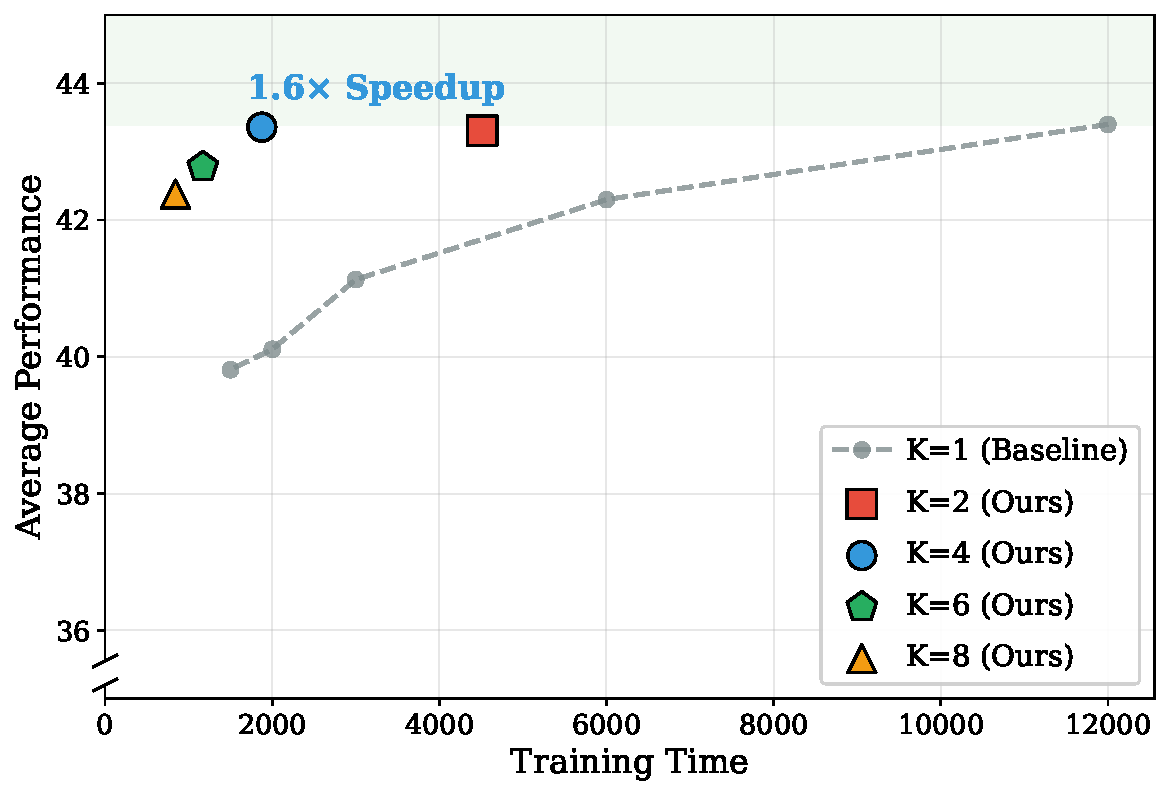
\includegraphics[width=0.9\linewidth]{figures/pareto_main.pdf}
\caption{Training efficiency: Time vs. Performance. The gray dashed line shows $K$=1 baseline performance at different training steps. Our method (colored markers) achieves better performance with significantly less training time.}
\label{fig:pareto_main}
\end{figure}

\paragraph{Ablations}

\begin{table*}[t]
\centering
\caption{Ablation study of complementary masking of \name{} in AR to Diffusion setting.}
\label{tab:ar2diff_complementary_ablation}
\scalebox{0.84}{
\begin{tabular}{lc|ccccccc|c}
\toprule
Method & Complementary & GSM8K & MATH & MMLU & GPQA & IFEval & MBPP & HumanEval & Avg.\\
\midrule
$K$=2 & \cmark & 63.43$_{\pm 1.75}$ & 30.96$_{\pm 0.19}$ & 50.73$_{\pm 0.77}$ & 26.49$_{\pm 0.46}$ & 41.03$_{\pm 1.39}$ & 50.06$_{\pm 1.25}$ & 40.45$_{\pm 3.46}$ & 43.31$_{\pm 0.25}$ \\
$K$=2 & \xmark & 63.36$_{\pm 1.56}$ & 30.10$_{\pm 0.30}$ & 50.91$_{\pm 0.15}$ & 26.41$_{\pm 0.78}$ & 42.82$_{\pm 1.08}$ & 49.42$_{\pm 1.78}$ & 43.29$_{\pm 2.20}$ & 43.76$_{\pm 0.10}$ \\
\midrule
$K$=4 & \cmark & 62.25$_{\pm 0.89}$ & 29.32$_{\pm 0.47}$ & 51.60$_{\pm 0.25}$ & 26.86$_{\pm 0.52}$ & 42.70$_{\pm 1.30}$ & 48.12$_{\pm 0.60}$ & 42.68$_{\pm 1.61}$ & 43.36$_{\pm 0.13}$ \\
$K$=4 & \xmark & 61.58$_{\pm 1.67}$ & 29.11$_{\pm 0.52}$ & 52.21$_{\pm 0.23}$ & 26.12$_{\pm 1.02}$ & 43.90$_{\pm 1.63}$ & 50.59$_{\pm 1.59}$ & 41.16$_{\pm 2.71}$ & 43.52$_{\pm 0.67}$ \\
\bottomrule
\end{tabular}
}
\end{table*}

\paragraph{Gradient Analysis}
We analyze the gradient norm per step for different $K$ settings to understand the optimization dynamics of our method.
As shown in Figure~\ref{fig:gradient_analysis}, we observe that larger $K$ values lead to lower gradient norms per step.
This is because when multiple mask patterns share the same clean context, the gradients from different masked views are aggregated and averaged, resulting in a more stable and smoothed gradient direction.
The reduced gradient variance per step allows for more consistent optimization, which partially explains why our method maintains competitive performance even with fewer training steps.

\begin{figure}[t]
\centering
% TODO: gradient analysis figure
\fbox{\parbox{0.8\linewidth}{\centering\vspace{2em}TODO: Gradient Norm Analysis Figure\vspace{2em}}}
\caption{Gradient norm per step with different $K$ values. Larger $K$ leads to lower gradient norm due to gradient averaging across multiple mask patterns.}
\label{fig:gradient_analysis}
\end{figure}

\subsection{Training Diffusion from Scratch}

For \textbf{Training Diffusion from Scratch}, we follow the experimental settings and framework established by SMDM~\citep{smdm}, using it as our baseline to demonstrate the effectiveness of our approach.

\paragraph{Models}

We train masked diffusion language models from scratch at three different scales: 170M, 336M, and 1028M parameters.
All models are trained on the SlimPajama~\citep{slimpajama} and StarCoder~\citep{starcoder} datasets.
We use a batch size of 256 and a context length of 2048 tokens.
The learning rate is set to $2e-4$ and the learning rate warmup is set to $1\%$ of the total training steps.

\paragraph{Benchmarks}

Following SMDM~\citep{smdm}, we use eight benchmarks covering commonsense reasoning and reading comprehension tasks, including
ARC-e~\citep{arc}, BoolQ~\citep{boolq}, Hellaswag~\citep{hellaswag}, Obqa~\citep{obqa}, PIQA~\citep{piqa}, RACE~\citep{race}, SIQA~\citep{siqa}, LAMBADA~\citep{lambada}.
All benchmarks are evaluated in the zero-shot setting.

\subsection{Speedup Analysis}

We analyze the computational speedup of our context-sharing attention mechanism at both the attention kernel level and the end-to-end training level.
To ensure a fair comparison, we fix the batch size to $4$ and the sequence length to $N = 2048$.
The baseline approach processes $K$ mask patterns independently, resulting in a batch size of $4K$ with sequence length $2N$.
In contrast, our method maintains the same batch size of $4$ but increases the sequence length to $(1+K)N$ by concatenating the shared clean text with $K$ masked texts.

\paragraph{Attention Kernel Speedup}
Our context-sharing attention mask is highly sparse: each masked segment only attends to the shared clean prefix and itself, while remaining isolated from other segments.
By leveraging FlexAttention~\citep{flexattention}, we exploit this sparsity pattern to achieve significant speedup in the attention computation.
As shown in Figure~\ref{fig:attention_speedup}, our sparse attention kernel achieves up to $TODO\times$ speedup compared to dense attention when the number of mask patterns $K$ increases.

\begin{figure}[t]
\centering
% TODO: attention speedup figure
\fbox{\parbox{0.8\linewidth}{\centering\vspace{2em}TODO: Attention Speedup Figure\vspace{2em}}}
\caption{Attention kernel speedup with different number of mask patterns $K$.}
\label{fig:attention_speedup}
\end{figure}

\paragraph{End-to-End Training Speedup}
We measure the end-to-end training speedup by comparing the wall-clock time per training step of our method against the baseline.
As shown in Figure~\ref{fig:e2e_speedup}, our method achieves $TODO\times$ end-to-end training speedup with $K=4$ mask patterns, demonstrating the practical efficiency gains of our approach.

\begin{figure}[t]
\centering
% TODO: end-to-end speedup figure
\fbox{\parbox{0.8\linewidth}{\centering\vspace{2em}TODO: End-to-End Speedup Figure\vspace{2em}}}
\caption{End-to-end training speedup with different number of mask patterns $K$.}
\label{fig:e2e_speedup}
\end{figure}
